\section{Применение метода}

Рассмотрим симметричные трехатомные гидриды $\ce{H2X}$. Они представляются хорошим объектом для изучения вращательной динамики и влияния колебательных движений на характер вращательного движения. В условиях высокого вращательного возбуждения легкие концевые атомы ставовятся подвижными, подвергаясь воздействию центробежных сил. Также, небольшое количество внутренних степеней свободы, делает эту систему доступной для изучения описанным методом. 

\subsection{Модель трехатомного гидрида с деформационной степенью свободы.}

В качестве первой системы рассмотрим простейшую модель симметричной трехатомной молекулы $\ce{H2X}$. В качестве первого \underline{упрощения} зафиксируем расстояния между легкими атомами и центральным атомом. Таким образом, колебательная динамика молекулярной системы сводится к колебанию ножничного типа. Также, будем считать, что масса тяжелого центрального атома много больше масс легких атомов (\underline{фактически, бесконечность}), что позволит нам поместить центр масс молекулярной системы на тяжелый атом. Несмотря на кажущуюся грубость описанной модели, она позволяет на качественном уровне описать колебательно-вращательное взаимодействие в трехатомных гидридах. Предложенная модель применима по причине того, что существенное влияние на колебательно-вращательное движение оказывает взаимодействие колебания деформационного типа с вращением молекулярной системы.

На рис.\eqref{fig:triatomic} молекула изображена в подвижной системе координат, причем ось $Ox$ параллельна биссектрисе валентного угла $q$, а ось $Oy$ перпендикулярна плоскости молекулы. Обозначим массу легких атомов -- $m$, расстояние между легким и тяжелым атомами -- $r_0$. 

\begin{figure}[!ht]
  \centering
	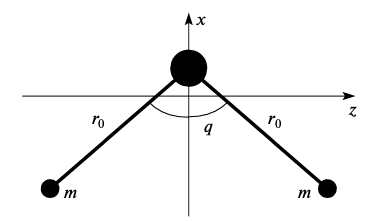
\includegraphics[width=0.4\textwidth]{../pictures/triatomic_fixed.png}
	\caption{Молекула $\ce{H2X}$ в подвижной системе отсчета.}
	\label{fig:triatomic}
\end{figure}

Выпишем координаты легких атомов в системе координат, связанной с центром масс.
\vverh
\begin{gather}
\left\{
\begin{aligned}
x_1 &= - r_0 \cos \lb \frac{q}{2} \rb \\
y_1 &= 0 \\
z_1 &= - r_0 \sin \lb \frac{q}{2} \rb 
\end{aligned}
\right. \quad \quad \quad
\left\{
\begin{aligned}
x_3 &= - r_0 \cos \lb \frac{q}{2} \rb \\
y_3 &= 0 \\
z_3 &= r_0 \sin \lb \frac{q}{2} \rb
\end{aligned}
\right.\notag
\end{gather}

Используя формулы, приведенные в предыдущей части, получим элементы матриц $\bba$, $\bbA$, $\bbI$, определяющих кинетическую энергию в форме Лагранжа в подвижной системе координат, учитывающей внутренние степени свободы. Размер матрицы $\bba$ равен $\dim \bba = s \times s$, где $s$ - количество внутренних степеней свободы, т.е. в данном случае матрица $\bba$ является числом: $\bba = \frac{I_0}{2}$, где $I_0 = m r_0^2$. Несложные преобразования показывают, что матрица $\bbA$ является нулевой. Тензор инерции рассматриваемой системы имеет диагональный вид, причем компоненты $I_{xx}$, $I_{zz}$ в сумме дают $I_{yy}$ (т.к. система плоская): $I_{xx} = 2 I_0 \sin^2 \lb \frac{q}{2} \rb$, $I_{yy} = 2I_0$, $I_{zz} = 2I_0 \cos^2 \lb \frac{q}{2} \rb$. Итак, кинетическая энергия 
в форме Лагранжа принимает следующий вид:
\vverh
\begin{gather}
T_\mathcal{L} = \frac{1}{2} \sum_i m_i \dot{\vec{R}}_i^2 + \vec{\Omega}^{\, \top} \sum_i m_i \left[ \vec{R}_i \times \dot{\vec{R}}_i \right] + \frac{1}{2} \vec{\Omega}^{\, \top} \bbI \ \vec{\Omega} = \frac{1}{2} \frac{I_0}{2} \dot{q}^2 + \frac{1}{2} \vec{\Omega}^{\, \top} \bbI \ \vec{\Omega}. \notag
\end{gather} 

Для перехода к кинетической энергии в форме Гамильтона применим формулы, полученные при помощи подхода Фробениуса к обращению блочных матриц. Т.к. $\bbA = \bbzero$: $\bbG_{11} = \bbI^{-1}$, $G_{12} = G_{21} = \bbzero$, $\bbG_{22} = \bba^{-1}$. Обращая матрицу тензора инерции и раскрывая матричное выражение в скалярное, получаем кинетическую энергию в Гамильтоновском представлении:
\vverh
\begin{gather}
T_\mathcal{H} = \frac{1}{2} \lb \frac{J_x^2}{I_{xx}} + \frac{J_y^2}{I_{yy}} + \frac{J_z^2}{I_{zz}} \rb + \frac{p^2}{I_0}, \notag
\end{gather}

В качестве потенциала, описывающего деформационное колебание, был взят потенциал Пешля-Теллера: $V = \frac{1}{2I_0} \lb \frac{V_{-}}{1 - \cos q} + \frac{V_{+}}{1 + \cos q} \rb$, где постоянные $V_{-}$, $V_{+}$ могут быть найдены исходя из равновесного значения угловой координаты $q_0$ и гармонической частоты деформационного колебания $\omega_0$:
\vverh
\begin{gather}
V_{\pm} = \frac{1}{4} I_0^2 \omega_0^2 (1 \pm \cos q_0 )^2. \notag
\end{gather}

Выбор потенциала обусловлен тем, что задача описания энергетического спектра квантового осциллятора с потенциалом этого типа допускает точное аналитическое решение:
\vverh
\begin{gather}
E_n = \frac{1}{I_0} \hbar^2 \left[ n + \frac{1}{2 \hbar} \lb \sqrt{V_{-}} + \sqrt{V_{+}} \rb \right] \times \left[ n + 1 + \frac{1}{2 \hbar} \lb \sqrt{V_{-}} + \sqrt{V_{+}} \rb \right], \quad n = 0, 1, 2, \dots \notag 
\end{gather}

%что переход к эффективному потенциалу не приводит к качественному изменению %потенциальных членов:

%\begin{gather}
%V_{eff.} = V(q) + \frac{1}{2I_0} \lb \frac{J_x^2}{1 - \cos q} + \frac{1}{2} J_y^2 + %\frac{J_z^2}{1 + \cos q}
%\end{gather} 
 